\documentclass[11pt]{article}

\usepackage{fullpage}
\usepackage{amsmath, amssymb, bm, cite, epsfig, psfrag}
\usepackage{graphicx}
\usepackage{float}
\usepackage{amsthm}
\usepackage{amsfonts}
\usepackage{listings}
\usepackage{cite}
\usepackage{hyperref}
\usepackage{tikz}
\usepackage{enumerate}
\usetikzlibrary{shapes,arrows}
%\usetikzlibrary{dsp,chains}

%\restylefloat{figure}
%\theoremstyle{plain}      \newtheorem{theorem}{Theorem}
%\theoremstyle{definition} \newtheorem{definition}{Definition}

\def\del{\partial}
\def\ds{\displaystyle}
\def\ts{\textstyle}
\def\beq{\begin{equation}}
\def\eeq{\end{equation}}
\def\beqa{\begin{eqnarray}}
\def\eeqa{\end{eqnarray}}
\def\beqan{\begin{eqnarray*}}
\def\eeqan{\end{eqnarray*}}
\def\nn{\nonumber}
\def\binomial{\mathop{\mathrm{binomial}}}
\def\half{{\ts\frac{1}{2}}}
\def\Half{{\frac{1}{2}}}
\def\N{{\mathbb{N}}}
\def\Z{{\mathbb{Z}}}
\def\Q{{\mathbb{Q}}}
\def\R{{\mathbb{R}}}
\def\C{{\mathbb{C}}}
\def\argmin{\mathop{\mathrm{arg\,min}}}
\def\argmax{\mathop{\mathrm{arg\,max}}}
%\def\span{\mathop{\mathrm{span}}}
\def\diag{\mathop{\mathrm{diag}}}
\def\x{\times}
\def\limn{\lim_{n \rightarrow \infty}}
\def\liminfn{\liminf_{n \rightarrow \infty}}
\def\limsupn{\limsup_{n \rightarrow \infty}}
\def\GV{Guo and Verd{\'u}}
\def\MID{\,|\,}
\def\MIDD{\,;\,}

\newtheorem{proposition}{Proposition}
\newtheorem{definition}{Definition}
\newtheorem{theorem}{Theorem}
\newtheorem{lemma}{Lemma}
\newtheorem{corollary}{Corollary}
\newtheorem{assumption}{Assumption}
\newtheorem{claim}{Claim}
\def\qed{\mbox{} \hfill $\Box$}
\setlength{\unitlength}{1mm}

\def\bhat{\widehat{b}}
\def\ehat{\widehat{e}}
\def\phat{\widehat{p}}
\def\qhat{\widehat{q}}
\def\rhat{\widehat{r}}
\def\shat{\widehat{s}}
\def\uhat{\widehat{u}}
\def\ubar{\overline{u}}
\def\vhat{\widehat{v}}
\def\xhat{\widehat{x}}
\def\xbar{\overline{x}}
\def\zhat{\widehat{z}}
\def\zbar{\overline{z}}
\def\la{\leftarrow}
\def\ra{\rightarrow}
\def\MSE{\mbox{\small \sffamily MSE}}
\def\SNR{\mbox{\small \sffamily SNR}}
\def\SINR{\mbox{\small \sffamily SINR}}
\def\arr{\rightarrow}
\def\Exp{\mathbb{E}}
\def\var{\mbox{var}}
\def\Tr{\mbox{Tr}}
\def\tm1{t\! - \! 1}
\def\tp1{t\! + \! 1}

\def\Xset{{\cal X}}

\newcommand{\one}{\mathbf{1}}
\newcommand{\abf}{\mathbf{a}}
\newcommand{\bbf}{\mathbf{b}}
\newcommand{\dbf}{\mathbf{d}}
\newcommand{\ebf}{\mathbf{e}}
\newcommand{\gbf}{\mathbf{g}}
\newcommand{\hbf}{\mathbf{h}}
\newcommand{\pbf}{\mathbf{p}}
\newcommand{\pbfhat}{\widehat{\mathbf{p}}}
\newcommand{\qbf}{\mathbf{q}}
\newcommand{\qbfhat}{\widehat{\mathbf{q}}}
\newcommand{\rbf}{\mathbf{r}}
\newcommand{\rbfhat}{\widehat{\mathbf{r}}}
\newcommand{\sbf}{\mathbf{s}}
\newcommand{\sbfhat}{\widehat{\mathbf{s}}}
\newcommand{\ubf}{\mathbf{u}}
\newcommand{\ubfhat}{\widehat{\mathbf{u}}}
\newcommand{\utildebf}{\tilde{\mathbf{u}}}
\newcommand{\vbf}{\mathbf{v}}
\newcommand{\vbfhat}{\widehat{\mathbf{v}}}
\newcommand{\wbf}{\mathbf{w}}
\newcommand{\wbfhat}{\widehat{\mathbf{w}}}
\newcommand{\xbf}{\mathbf{x}}
\newcommand{\xbfhat}{\widehat{\mathbf{x}}}
\newcommand{\xbfbar}{\overline{\mathbf{x}}}
\newcommand{\ybf}{\mathbf{y}}
\newcommand{\zbf}{\mathbf{z}}
\newcommand{\zbfbar}{\overline{\mathbf{z}}}
\newcommand{\zbfhat}{\widehat{\mathbf{z}}}
\newcommand{\Ahat}{\widehat{A}}
\newcommand{\Abf}{\mathbf{A}}
\newcommand{\Bbf}{\mathbf{B}}
\newcommand{\Cbf}{\mathbf{C}}
\newcommand{\Bbfhat}{\widehat{\mathbf{B}}}
\newcommand{\Dbf}{\mathbf{D}}
\newcommand{\Gbf}{\mathbf{G}}
\newcommand{\Hbf}{\mathbf{H}}
\newcommand{\Kbf}{\mathbf{K}}
\newcommand{\Pbf}{\mathbf{P}}
\newcommand{\Phat}{\widehat{P}}
\newcommand{\Qbf}{\mathbf{Q}}
\newcommand{\Rbf}{\mathbf{R}}
\newcommand{\Rhat}{\widehat{R}}
\newcommand{\Sbf}{\mathbf{S}}
\newcommand{\Ubf}{\mathbf{U}}
\newcommand{\Vbf}{\mathbf{V}}
\newcommand{\Wbf}{\mathbf{W}}
\newcommand{\Xhat}{\widehat{X}}
\newcommand{\Xbf}{\mathbf{X}}
\newcommand{\Ybf}{\mathbf{Y}}
\newcommand{\Zbf}{\mathbf{Z}}
\newcommand{\Zhat}{\widehat{Z}}
\newcommand{\Zbfhat}{\widehat{\mathbf{Z}}}
\def\alphabf{{\boldsymbol \alpha}}
\def\betabf{{\boldsymbol \beta}}
\def\mubf{{\boldsymbol \mu}}
\def\lambdabf{{\boldsymbol \lambda}}
\def\etabf{{\boldsymbol \eta}}
\def\xibf{{\boldsymbol \xi}}
\def\taubf{{\boldsymbol \tau}}
\def\sigmahat{{\widehat{\sigma}}}
\def\thetabf{{\bm{\theta}}}
\def\thetabfhat{{\widehat{\bm{\theta}}}}
\def\thetahat{{\widehat{\theta}}}
\def\mubar{\overline{\mu}}
\def\muavg{\mu}
\def\sigbf{\bm{\sigma}}
\def\etal{\emph{et al.}}
\def\Ggothic{\mathfrak{G}}
\def\Pset{{\mathcal P}}
\newcommand{\bigCond}[2]{\bigl({#1} \!\bigm\vert\! {#2} \bigr)}
\newcommand{\BigCond}[2]{\Bigl({#1} \!\Bigm\vert\! {#2} \Bigr)}

\def\Rect{\mathop{Rect}}
\def\sinc{\mathop{sinc}}
\def\Real{\mathrm{Re}}
\def\Imag{\mathrm{Im}}



\begin{document}

\title{Problems:  Passband Modulation}
\author{Prof.\ Sundeep Rangan}
\date{}

\maketitle

\begin{enumerate}

\item \emph{Passband conversion.}
Let $u(t)$ be a complex baseband signal with the real and imaginary parts of
 the spectrum (Fourier Transform) shown in
Fig.~\ref{fig:Ubb}.  The constants are $f_0 = $ 5 MHz, $f_1 = $ 10 MHz, $A=8$ and $B=10$.

\begin{figure}[h]
\center
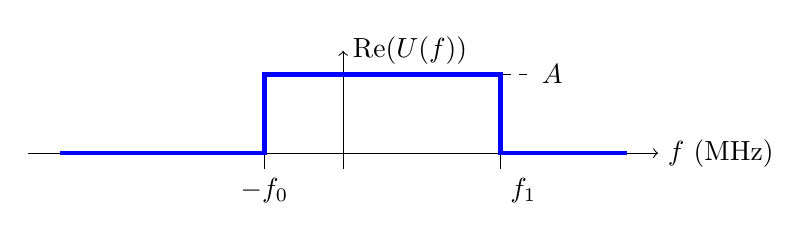
\begin{tikzpicture}[xscale=2,yscale=1]
    \pgfmathsetmacro{\fa}{-0.5}
    \pgfmathsetmacro{\fb}{1}
    \pgfmathsetmacro{\fm}{2}
    \pgfmathsetmacro{\A}{1}
    \pgfmathsetmacro{\tic}{0.2}

    % Draw the axes
    \draw [->] (-\fm,0) -- (\fm,0) node [right] {$f$ (MHz)};
    \draw [->] (0,-\tic) -- (0,1.3) node [right] {$\Real(U(f))$};
    \draw [-] (\fa,\tic) -- (\fa,-\tic) node [below] {$-f_0$};
    \draw [-] (\fb,\tic) -- (\fb,-\tic) node [below right] {$f_1$};
    \draw [-,dashed] (\fb-\tic,\A) -- (\fb+\tic,\A) node [right] {$A$};

    % Draw Real U(f)
    \draw [ultra thick,blue,-] (-\fm+0.2,0) -- (\fa,0) -- (\fa,\A) --
         (\fb,\A) -- (\fb,0) -- (\fm-0.2,0);

\end{tikzpicture}

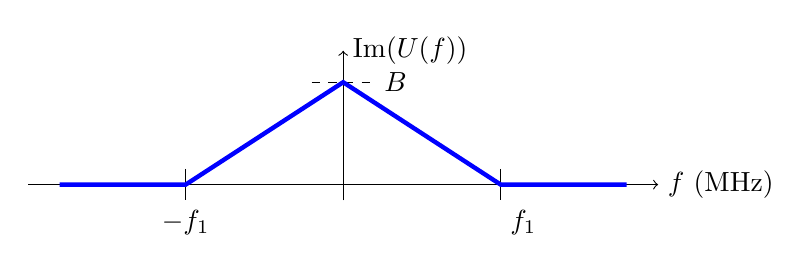
\begin{tikzpicture}[xscale=2,yscale=1]
    \pgfmathsetmacro{\fa}{-0.5}
    \pgfmathsetmacro{\fb}{1}
    \pgfmathsetmacro{\fm}{2}
    \pgfmathsetmacro{\A}{1.3}
    \pgfmathsetmacro{\tic}{0.2}

    % Draw the axes
    \draw [->] (-\fm,0) -- (\fm,0) node [right] {$f$ (MHz)};
    \draw [->] (0,-\tic) -- (0,1.7) node [right] {$\Imag(U(f))$};
    \draw [-] (-\fb,\tic) -- (-\fb,-\tic) node [below] {$-f_1$};
    \draw [-] (\fb,\tic) -- (\fb,-\tic) node [below right] {$f_1$};
    \draw [-,dashed] (-\tic,\A) -- (\tic,\A) node [right] {$B$};

    % Draw Imag U(f)
    \draw [ultra thick,blue,-] (-\fm+0.2,0) -- (-\fb,0) -- (0,\A)
          -- (\fb,0) -- (\fm-0.2,0);

\end{tikzpicture}

\caption{Real and imaginary parts of complex baseband signal $U(f)$} \label{fig:Ubb}
\end{figure}

\begin{enumerate}[(a)]


\item Suppose that we create a real passband signal $u_p(t) = \Real(u(t)e^{2\pi if_c t})$
for a carrier frequency $f_c = 800$ MHz.  Draw the spectrum of $U_p(f)$.  Show
 both the real and imaginary parts and show both the positive and negative frequencies.

\item Is $u(t)$ an energy signal or power signal?  What is its energy or power (in linear scale)?
Leave your answer in terms of $A$, $B$, $f_0$ and $f_1$.  You do not need to
convert to dB scale.

\item A receiver attempts to downcovert the signal with a two step process:
\[
    v(t)= 2u(t)e^{-2\pi i f_c t}, \quad \hat{u}(t) = h_{LPF}(t) * v(t),
\]
where $h_{LPF}(t)$ has a frequency response,
\[
    H_{LPF}(f) = \begin{cases}
        C & \mbox{if } |f| < f_{LPF} \\
        0 & \mbox{if } |f| \geq f_{LPF}.
        \end{cases}
\]
For what values of $C$ and $f_{LPF}$ is $\hat{u}=u(t)$?
\end{enumerate}

\item \emph{Baseband equivalent filter.}
Consider a communication system with three steps:
\begin{itemize}
\item A complex baseband signal $u(t)$ is upconverted $u_p(t)=\Real(u(t)e^{2\pi if_ct})$
for some $f_c$.
\item The real passband channel is passed through a linear filter,
\[
    \frac{dy_p(t)}{dt} = b u_p(t)- ay_p(t),
\]
with constants $a$ and $b>0$.
\item The received signal is downconverted, $v(t)=2y_p(t)e^{-2\pi i f_ct}$ and
$y(t)=h_{\rm LPF}(t)*v(t)$ where $h_{\rm LPF}(t)$ is an ideal low-pass filter.
\end{itemize}
\begin{enumerate}[(a)]
\item What is the real passband frequency response, $H_p(f) = \frac{Y_p(f)}{U_p(f)}$?

\item What is the effective baseband frequency response $H(f) = \frac{Y(f)}{U(f)}$?

\item Find $a_1$ and $b_1$ such that
\[
    \frac{dy(t)}{dt} = b_1 x(t)- a_1y(t).
\]

\item Suppose that $2\pi f_c \gg a$, what is the power gain of $H(0)$ in dB?
\end{enumerate}

\item \emph{PSD and RX filtering.}
Suppose that a real passband signal has two components:
\[
    x(t)=x_0(t)+x_1(t),
\]
where $x_0(t)$ is a desired signal, and $x_1(t)$ is an interfering signal.  They have PSD
$S_i(f)=A_i\Rect((f-f_i)/W_i)$, $i=0,1$ with parameters:
\begin{itemize}
\item Desired signal: $f_0 = 2.50$ GHz, $W_0 = $ 20~MHz, total receive power $P_0$ = -100~dBm.
\item Interfering signal: $f_1 = 2.53$ GHz, $W_1 = $ 10~MHz, total receive power $P_1$ = -80~dBm.
\end{itemize}
\begin{enumerate}[(a)]
\item Find $A_i$ from $P_i$ using reasonable approximations.  State the units of $A_i$.
\item Draw $S_0(f)$ and $S_1(f)$.
\item A signal is downconverted with mixing $v(t)=2x(t)e^{2\pi i f_ct}$ and $u(t)=h(t)*v(t)$.
Find $f_c$ and a filter magnitude response $|H(f)|^2$ such that:
\begin{itemize}
\item The component from desired signal is centered at 0 and amplified to -60 dBm.
\item The component from interfering signal attenuated to below -110 dBm.
\end{itemize}
There is no single correct answer.  Draw $|H(f)|^2$ and the PSD of $u(t)$.
\end{enumerate}


\end{enumerate}

\end{document}
